%! alt A 5 by 5 field of 1 m square plots. Six plots are left empty and shaded: the centre plot, the four plots diagonally next to it, and the middle plot of the bottom edge. No two empty plots share a side. The fencing, highlighted, runs round the outside of the field except along the bottom side of the empty edge plot, and round each of the five inner empty plots. It has length 22 + 5 times 4 = 42 metres.
%! after_paragraph 2
%! scale 1
% The shared preamble of every Cevian figure. pipeline/figures turns these colours into theme-aware paint,
% and refuses any other colour, so draw only with them:
%   figink (lines and labels), figaux (construction lines), figaccent (the object the argument turns on),
%   figtint and figaccenttint (light fills).
\documentclass[border=1.5pt]{standalone}
\usepackage{tkz-euclide}
\definecolor{figink}{RGB}{0,0,0}
\definecolor{figaux}{RGB}{85,85,85}
\definecolor{figaccent}{RGB}{192,57,43}
\definecolor{figtint}{RGB}{221,221,221}
\definecolor{figaccenttint}{RGB}{245,213,208}
% tkz-euclide's defaults draw circles, compasses and marks in 50% grey and fill points with a tint.
\makeatletter
\def\tkz@otherlinecolor{figink}
\def\tkz@euc@circlecolor{figink}
\def\tkz@euc@compasscolor{figink}
\def\tkz@euc@mkcolor{figink}
\def\tkz@mk@fill{figink}
\def\tkz@euc@pointfillcolor{figink}
\makeatother
\tkzSetUpLine[color=figink,line width=.7pt]
\tkzSetUpArc[color=figink,line width=.7pt]
\tkzSetUpCompass[color=figink,line width=.5pt]
\tkzSetUpPoint[color=figink,fill=figink,size=3.1pt]
\tikzset{
  every picture/.style={line cap=round,line join=round,color=figink},
  circle style/.append style={color=figink,line width=.7pt},
  aux/.style={color=figaux,line width=.45pt,dash pattern=on 2.6pt off 2pt},
  key/.style={color=figaccent,line width=1pt},
  mk/.style={color=figink,line width=.5pt},
  lbl/.style={color=figink,inner sep=2.2pt},
  len/.style={color=figink,inner sep=1.5pt,font=\small},
}

\begin{document}
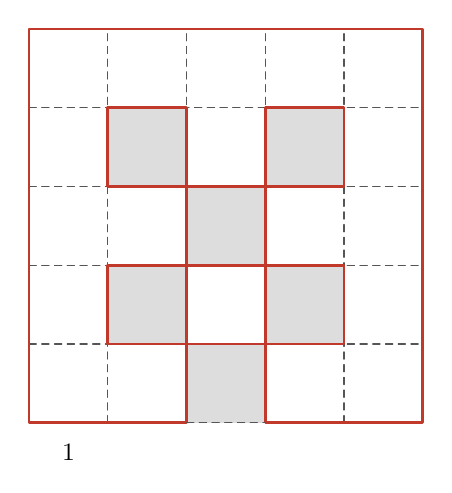
\begin{tikzpicture}
\tkzDefPoint(0.0,0.0){P00} %! P00 = (0, 0)
\tkzDefPoint(0.0,1.0000000){P01} %! P01 = (0, 1)
\tkzDefPoint(0.0,2.0000000){P02} %! P02 = (0, 2)
\tkzDefPoint(0.0,3.0000000){P03} %! P03 = (0, 3)
\tkzDefPoint(0.0,4.0000000){P04} %! P04 = (0, 4)
\tkzDefPoint(0.0,5.0000000){P05} %! P05 = (0, 5)
\tkzDefPoint(1.0000000,0.0){P10} %! P10 = (1, 0)
\tkzDefPoint(1.0000000,1.0000000){P11} %! P11 = (1, 1)
\tkzDefPoint(1.0000000,2.0000000){P12} %! P12 = (1, 2)
\tkzDefPoint(1.0000000,3.0000000){P13} %! P13 = (1, 3)
\tkzDefPoint(1.0000000,4.0000000){P14} %! P14 = (1, 4)
\tkzDefPoint(1.0000000,5.0000000){P15} %! P15 = (1, 5)
\tkzDefPoint(2.0000000,0.0){P20} %! P20 = (2, 0)
\tkzDefPoint(2.0000000,1.0000000){P21} %! P21 = (2, 1)
\tkzDefPoint(2.0000000,2.0000000){P22} %! P22 = (2, 2)
\tkzDefPoint(2.0000000,3.0000000){P23} %! P23 = (2, 3)
\tkzDefPoint(2.0000000,4.0000000){P24} %! P24 = (2, 4)
\tkzDefPoint(2.0000000,5.0000000){P25} %! P25 = (2, 5)
\tkzDefPoint(3.0000000,0.0){P30} %! P30 = (3, 0)
\tkzDefPoint(3.0000000,1.0000000){P31} %! P31 = (3, 1)
\tkzDefPoint(3.0000000,2.0000000){P32} %! P32 = (3, 2)
\tkzDefPoint(3.0000000,3.0000000){P33} %! P33 = (3, 3)
\tkzDefPoint(3.0000000,4.0000000){P34} %! P34 = (3, 4)
\tkzDefPoint(3.0000000,5.0000000){P35} %! P35 = (3, 5)
\tkzDefPoint(4.0000000,0.0){P40} %! P40 = (4, 0)
\tkzDefPoint(4.0000000,1.0000000){P41} %! P41 = (4, 1)
\tkzDefPoint(4.0000000,2.0000000){P42} %! P42 = (4, 2)
\tkzDefPoint(4.0000000,3.0000000){P43} %! P43 = (4, 3)
\tkzDefPoint(4.0000000,4.0000000){P44} %! P44 = (4, 4)
\tkzDefPoint(4.0000000,5.0000000){P45} %! P45 = (4, 5)
\tkzDefPoint(5.0000000,0.0){P50} %! P50 = (5, 0)
\tkzDefPoint(5.0000000,1.0000000){P51} %! P51 = (5, 1)
\tkzDefPoint(5.0000000,2.0000000){P52} %! P52 = (5, 2)
\tkzDefPoint(5.0000000,3.0000000){P53} %! P53 = (5, 3)
\tkzDefPoint(5.0000000,4.0000000){P54} %! P54 = (5, 4)
\tkzDefPoint(5.0000000,5.0000000){P55} %! P55 = (5, 5)
\tkzDefPoint(0.50000000,-0.38000000){Lone} %! Lone = (0.5, -0.38)
%! fact dist(P00, P50) == 5
%! fact dist(P00, P05) == 5
%! fact dist(P20, P00) + dist(P00, P05) + dist(P05, P55) + dist(P55, P50) + dist(P50, P30) + dist(P30, P31) + dist(P31, P21) + dist(P21, P20) + 4*dist(P11, P21) + 4*dist(P13, P23) + 4*dist(P22, P32) + 4*dist(P31, P41) + 4*dist(P33, P43) == 42
\tkzFillPolygon[color=figtint](P11,P21,P22,P12)
\tkzFillPolygon[color=figtint](P13,P23,P24,P14)
\tkzFillPolygon[color=figtint](P22,P32,P33,P23)
\tkzFillPolygon[color=figtint](P31,P41,P42,P32)
\tkzFillPolygon[color=figtint](P33,P43,P44,P34)
\tkzFillPolygon[color=figtint](P20,P30,P31,P21)
\tkzDrawSegments[aux](P10,P15 P20,P25 P30,P35 P40,P45 P01,P51 P02,P52 P03,P53 P04,P54)
\tkzDrawPolygon[key](P20,P00,P05,P55,P50,P30,P31,P21)
\tkzDrawPolygon[key](P11,P21,P22,P12)
\tkzDrawPolygon[key](P13,P23,P24,P14)
\tkzDrawPolygon[key](P22,P32,P33,P23)
\tkzDrawPolygon[key](P31,P41,P42,P32)
\tkzDrawPolygon[key](P33,P43,P44,P34)
\tkzDrawSegment[aux](P20,P30)
\tkzLabelPoint[anchor=center,len](Lone){$1$}
\end{tikzpicture}
\end{document}
